\documentclass[11pt]{report}
\title{Experiments with Buffer Overflows \\ 
    \textbf{Segurança de Software}}
\author{
Guilherme Santos    \\
\texttt{fc62533}  \and
Inês Rocha       \\
\texttt{fc62699}  \and
Miguel Mota   \\ 
\texttt{fc62702}
}
\date{\today}

\usepackage[left=1in,right=1in,top=1in,bottom=1in]{geometry}
\usepackage{tikz,pgfplots}
\usepackage{subfig}
\usepackage{caption}
\usepackage{amsmath}
\begin{document}

\maketitle


\section*{Heap Overflow}

1 (d) O heap cresce de baixo para cima, como foi feito o \texttt{malloc()} do \texttt{str} 
primeiro do que o do \texttt{critical}, o \texttt{str} vai aparecer em endereços menores do que os do \texttt{critical}. \\

\noindent1 (e) Como o \texttt{argv[1]} começa no endereço \texttt{0x555555756260}, fizemos a subtração do endereço 
\texttt{0x55555575627f} com o endereço anterior para sabermos o nº de caracteres antes de \texttt{'CIENCIAS'}.
Foram necessários 31 1's, o input foi \texttt{11111111111111111111111111111111CIENCIAS}.

\vspace{20pt}
\begin{figure}[h]
    \centering
    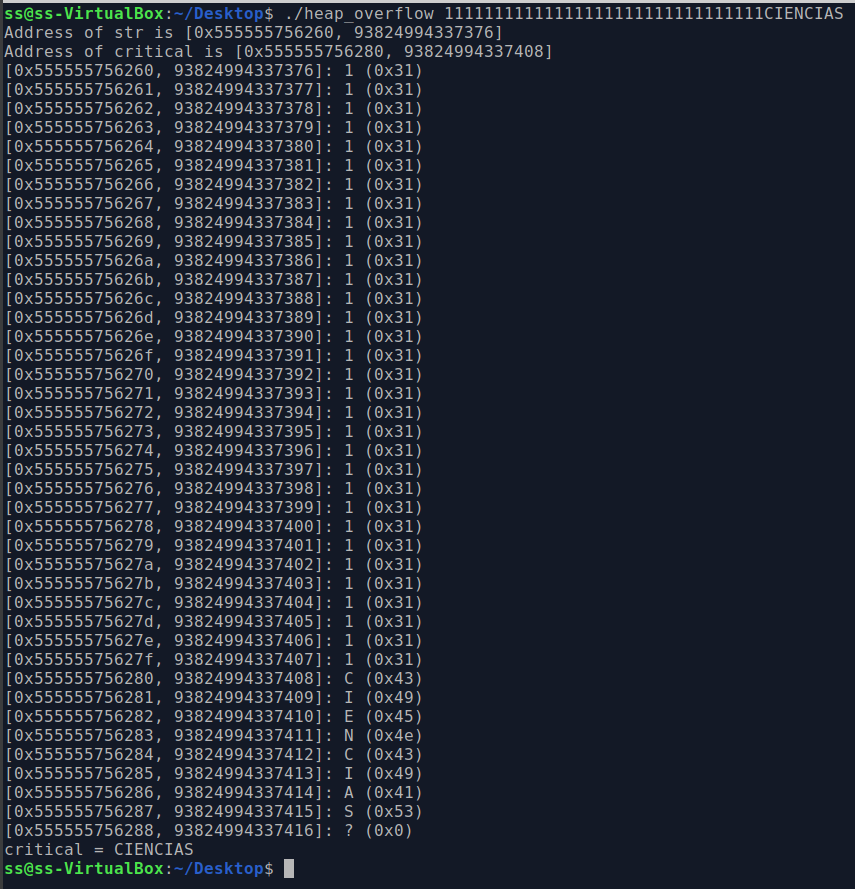
\includegraphics[width=0.7\textwidth]{ciencias.png}
    \caption{Output heap\_oveflow}
  \end{figure}

\pagebreak

\section*{Stack Overflow}

2(c) São necessários, no mínimo, 13 bytes (incluindo o null-terminator) para criar overflow no \texttt{buf}. Houve um overflow no RBP, 
como demonstrado no primeiro comando na figura abaixo e um overflow no RIP com 21 bytes, 
como demonstrado no segundo comando. 
Na segunda execução não foi impresso “I’m OK!” pois o RIP foi alterado e não voltou ao \texttt{main()} para fazer o \texttt{printf()}.

\vspace{20pt}
\begin{figure}[h]
    \centering
    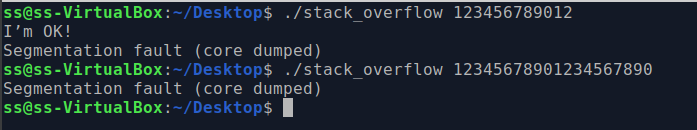
\includegraphics[width=0.5\textwidth]{rip.png}
    \caption{Output stack\_oveflow}
  \end{figure}

\vspace{20pt}

\noindent2(h) O programa não imprimiu a frase porque a função \texttt{cannot()} nunca é executada.
\\


\noindent2(j) São necessários 21 bytes (12 do buffer e 8 do RBP + 1) para dar overflow no RIP.
Foi escrito o endereço da função \texttt{cannot()} do fim até ao início, de baixo para cima pois quando o RIP lê o endereço, como é hexadecimal, interpreta-o ao contrário.
\texttt{0x55555555471a} → Endereço da função \texttt{cannot()}.

\vspace{20pt}

\begin{figure}[h]
    \centering
    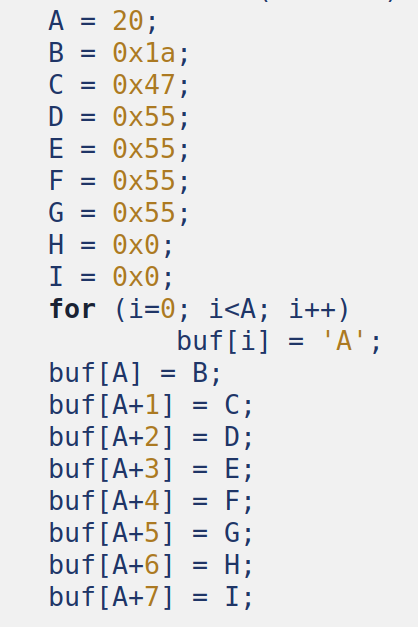
\includegraphics[width=0.3\textwidth]{valores.png}
    \caption{Valores}
  \end{figure}

\begin{figure}[h]
    \centering
    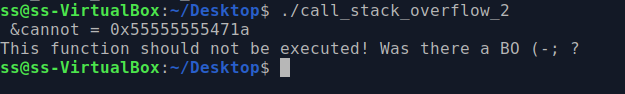
\includegraphics[width=0.4\textwidth]{BO_CALL.png}
    \caption{Execução de \texttt{cannot()}}
  \end{figure}

\vspace{20pt}

\end{document}